%#!platex main

\chapter{意味解析}

プログラミング言語の構文上の制約には、文脈自由文法の枠から外れるものがい
くつかある。ここまでにもところどころで述べてきたが、整理してみよう。
\begin{itemize}
 \item 変数の宣言は、その変数を使用するより先に出現しなくてはならない。
       \ref{110128_3Apr06}節でも述べた通り、これは文脈自由文法では表現で
       きない。もちろんLL(1)文法でも表現できない。
       \label{132708_10Apr06}
 \item 型の整合性。例えばC言語の\icode{int x = 10.0 + 2;}という文は、
       \icode{int x = (int)(10.0 + (float)2);}、つまり、(1)右辺の2が
       float型に変換され (2) 10.0 + 2.0 を計算し(結果は float 型)(3)
       int型に変換されて変数 x に代入される、というように計算される。これ
       らの型変換は、C言語の文法では表現されておらず、字句解析部や構文解
       析部では扱えない。
\end{itemize}

このように、文脈自由文法から外れる制約の検査や解析は、構文解析部の後で行
われる。これを{\bf 意味解析}(semantic analysis)という。意味解析は、構文
解析の出力である解析木を入力とし、その解析木を変形したり、別のデータ構造
を作成したりする。本章では、意味解析の基礎となる技術である翻訳スキームに
ついて述べ、いくつかの制約の検査について実例により説明する。

\section{記号表}

原始プログラム中でなんらかの名前がついている構成要素(変数名、関数名、構
造体、構造体のメンバなど)を特徴づける情報には次のようなものがある。
\begin{itemize}
 \item 構成要素の種類(変数、関数など)
 \item 構成要素の名前
 \item 型情報(変数の型、関数の引数の個数、個々の引数の型、返り値の型な
       ど)
 \item 属性(\icode{static}など)
 \item 構成要素が割り当てられている番地
\end{itemize}
これらの情報はコンパイラの各段階で頻繁に参照されるので、何らかの形のデー
タ構造で表現し、コンパイラ中で保持・管理しなければならない。コンパイラで
は通常、これらの情報を{\bfseries 記号表}(symbol table)という表で管理する。

\subsection{記号表の実装}

記号表を実装する最も簡単な方法は、構造体の配列を用いるものである。簡単の
ため、記号表に格納される情報を、識別子の文字列(\icode{lexname}、最大長さ
\icode{MAXLEN})、識別子のトークンの種類(\icode{lextoken})の2つであると
し、記号表に登録できるエントリの最大数を\icode{MAXENT}としておこう。する
と、記号表を表すデータ構造は次のようになる。

\begin{lstlisting}
typedef struct table_ent {
  char lexname[MAXLEN];
  int lextoken;
};
table_ent lextable[MAXENT];
\end{lstlisting}

記号表に対する主な操作は次の2つである。
\begin{itemize}
 \item \icode{int insert(char *s, int t)}…文字列$s$, トークン$t$のエント
       リを新たに記号表に登録し、そのエントリの番号(添字)を返す。すでに
       登録されていれば(登録できないとして)-1 を返す。
 \item \icode{int lookup(char *s)}…文字列$s$のエントリが記号表に登録され
       ているか調べる。あればそのエントリの番号(添字)を返し、なければ
       -1 を返す。
\end{itemize}

上記の構造体の配列による記号表に対し、これらの操作をC言語で実装することは
容易であろう。各自で試みられたい。

実際のコンパイラでは、上で示した記号表の実装は次のような問題がある。
\begin{enumerate}
 \item 登録できる文字列の長さに制限がある。つまり、プログラムで使える識
       別子の長さに制限がある。
       \label{141846_30Mar06}
 \item 記号表のエントリ数に制限がある。つまり、プログラムで使える識別子
       の数に制限がある。
       \label{141856_30Mar06}
 \item 記号表を検索したり、挿入しようとするエントリがあるかどうか調べる
       のに、最悪、記号表のエントリをすべて調べなければならない。つまり、
       insertやlookupの処理の効率が悪い。
       \label{141901_30Mar06}
\end{enumerate}

\ref{141846_30Mar06}は、\icode{lexname}を\icode{char}の固定長配列ではなく、
\icode{malloc()}などにより動的確保するようにすればよい。また
\ref{141856_30Mar06}は、配列ではなく連結リストなどを用いれば解決可能であ
る。しかし、\ref{141901_30Mar06}についてはこのような工夫では解決できず、
{\bfseries ハッシュ}法などの手法が必要になる\footnote{ハッシュ法について
は「アルゴリズム論」で取り上げられているので、説明は省略する。詳細は「ア
ルゴリズム論」の教科書\cite{エイホ77}を参照されたい。}。

\subsection{記号表による意味解析}

記号表を用いると、本章の最初で述べた構文上の制約「変数の宣言は、その変数
を使用するより先に出現しなくてはならない」は容易に検査できる。すなわち、
次のようにすればよい。
\begin{enumerate}
 \item 変数や関数、構造体などの宣言が出現したときに、名前、型などの情報を
       記号表に登録する。
 \item 予約語以外の識別子がプログラム中で出現したときに、記号表を参照し、
       その識別子がすでに登録されているか調べる。登録されていなければ、識
       別子の宣言をせずに使用されているので、誤りである。
\end{enumerate}

ここで注意をしておかなければならないのが、変数や関数などの{\bfseries 有効
範囲}(scope)、すなわちその変数や関数を参照することのできるプログラムの
範囲である。C言語の識別子には、有効範囲に関して次のような制限がある。
\begin{enumerate}
 \item 大域変数(global variable)、関数、構造体、構造体のメンバなどは、
       それが宣言された場所からファイルの終わりまでが有効範囲である。
       \label{144539_10Apr06}
 \item 関数の引数は、その関数の内部が有効範囲である。
       \label{144557_10Apr06}
 \item 関数内で宣言された変数(局所変数、local variable)は、宣言された場
       所からその関数の終わりまでが有効範囲である。
       \label{144603_10Apr06}
 \item 同じ識別子が大域変数と局所変数・引数としてともに用いられていた場合、
       局所変数・引数が優先する。
\end{enumerate}
記号表の管理も、この有効範囲を考慮して行わなければならない。

簡単なのは、\ref{144539_10Apr06}のタイプの識別子と、
\ref{144557_10Apr06}, \ref{144603_10Apr06}のタイプの識別子を別の記号表で
管理する、という方法である。記号表の管理は次のように修正される。ただし以
下では、それぞれの記号表を大域記号表、局所記号表と呼んでいる。
\begin{enumerate}
 \item 大域変数、構造体、構造体のメンバ、\icode{extern}文による(ファイル
       外部の変数、関数などの)宣言などが出現したときには、その名前、型な
       どの情報を大域記号表に登録する。
 \item 関数宣言が出現したときには、関数名とその型などの情報を大域記号表に、
       引数の名前、型などの情報を局所記号表にそれぞれ登録する。
 \item 局所変数の宣言が出現したときには、その変数の名前、型などの情報を局
       所記号表に登録する。
 \item 予約語以外の識別子がプログラム中で出現したときに、局所記号表、大域
       記号表の順に参照し、その識別子がすでに登録されているか調べる。どち
       らの記号表にも登録されていなければ、識別子の宣言をせずに使用されて
       いるので、誤りである。
 \item 関数宣言の終わりに到達すると、局所記号表の内容をすべて消去する。
\end{enumerate}

なお、C言語では、有効範囲として(中括弧で囲まれた)ブロックも考慮しなけれ
ばならない。また、\icode{goto}文の飛び先を指定するラベルも、上に述べたも
のとは異なる有効範囲を持っている。このような理由により、実際には、より複
雑な記号表管理が必要になる。また、「計算機言語I」で取り上げたMLや「計算機
言語II」で取り上げる予定のJavaなど、Cより複雑な有効範囲を持つプログラミン
グ言語でも、より複雑な記号表管理が必要である。

\section{型検査と型変換}
\label{163428_10Apr06}

次に、本章の最初に挙げた構文上の制約のうち、型の整合性について述べる。

「計算機言語I」で取り上げたMLでは、演算数に対する型の制限が非常に強い。例
えば、算術式$x\ \icode{div}\ y$であれば、$x, y$はいずれも整数型(\icode{int})
でなければならない。この制約は、\ref{190545_30Mar06}節の例と同様、以下の
ようなプログラム断片付き生成規則で表現することができる。
\begin{align*}
 list \rightarrow list\ \icode{div}\ digit &\ \{ \mbox{$list_l.type$ = }\\
 &\  \mbox{if ($list_r.type == int$ \&\& $digit.type == int$)} \\
 &\  \mbox{then $int$ else 型エラー} \} \\
 list \rightarrow digit & \ \{ list.type = digit.type; \} \\
 digit \rightarrow 0 & \ \{ digit.type = int; \} \\
 \cdots \\
 digit \rightarrow 9 & \ \{ digit.type = int; \} \\
\end{align*}

\ref{190545_30Mar06}節の算術式の値の計算と同様、この型検査は、プログラム
断片付き解析木を作り、それを深さ優先でたどりながらプログラム断片を実行す
ることで、処理できる。

C言語の場合も上の例と同様に型検査を行うことができる。ただし、原子型の種類
が多く(\icode{int}, \icode{signed int}, \icode{unsigned int},
\icode{long}, \icode{signed long}, \icode{unsigned long}, \icode{short},
$\cdots$)、かつ型の整合性に関するルールが複雑である。例えば$x + y$におい
て、$x$が\icode{float}型で$y$が\icode{int}型であっても誤りではない。この
場合、$y$が\icode{float}型に変換されてから加算が行われ、結果は
\icode{float}型になる\footnote{算術演算における演算数の型変換については
\cite{カーニハン89}のA6.5節を参照のこと。}。このとき、$y$に関する型変換は
プログラム実行時に行われることに注意しなければならない。つまり、コンパイ
ラは、$x$と$y$の加算の機械語命令に加え、$y$を\icode{float}に変換する機械
語命令を生成しなければならない。そのため、意味解析部では、$y$を
\icode{float}に変換する必要があるという情報を解析木に追加する(図
\ref{191552_10Apr06})。

\begin{figure}
 \begin{center}
  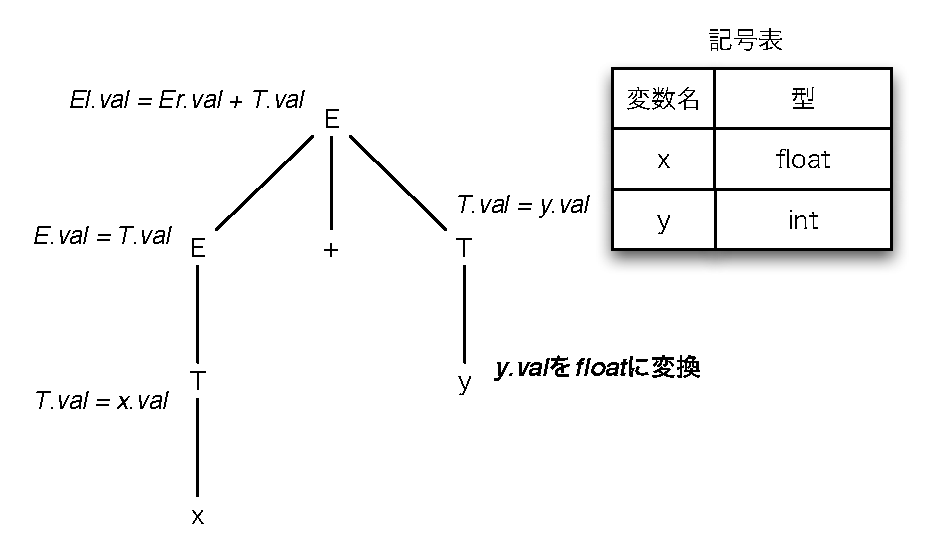
\includegraphics[width=12cm]{figure/type_conversion.pdf}
 \end{center}
 \caption{解析木への型変換情報の付加}
 \label{191552_10Apr06}
\end{figure}

\section{解析木を用いた意味解析}

解析木を用いると、さまざまな実用的な処理が体系的に行えるようになる。
\ref{163428_10Apr06}節で挙げた型検査や\ref{190545_30Mar06}節で述べた算術
式の値の計算がその例である。本節では、このような解析木を用いた意味解析の
基礎となる理論として、翻訳スキームという考え方を紹介する。

まず、コンパイラの動作に近い例として、中置記法で書かれた算術式を後置記法
に変換することを考えよう。

\subsection{中置記法と後置記法}

我々が普段目にする2項演算子は、たいてい、2つの演算数の間に演算子を書く。
\icode{32 + 9}, \icode{4 / 2}といった具合である。これを{\bfseries 中置記
法}(infix notation)という。しかし、算術式の書き方はこれだけではない。演
算子を2つの演算数の前に置く{\bfseries 前置記法}(prefix notation)、2 つ
の演算数の後ろに置く{\bfseries 後置記法}(postfix notation)という書き方
もある。ここでは後置記法のみもう少し詳しく説明することにしよう。

\begin{definition}
 中置記法による式$E$の後置記法は次のように再帰的に定義される。
 \begin{enumerate}
  \item $E$が変数または定数であれば、$E$の後置記法は$E$である。
  \item 任意の2項演算子$\op$について、$E_1 \op E_2$の後置記法は
	$E_1'~E_2'~\op$である。ここで$E_1', E_2'$はそれぞれ$E_1, E_2$の後
	置記法である。
  \item $(E)$の後置記法は$E'$である。ここで$E'$は$E$の後置記法である。
 \end{enumerate}$\Box$
\end{definition}

\begin{example}
 $32 + 3$の後置記法は$32~3~+$である。$9 + 4 * 3$の後置記法は$9~4~3~*~+$で
 ある。$(1+2)*4$の後置記法は$1~2~+~4~*$である。$\Box$
 \label{ex:prefix_notation}
\end{example}

後置記法で書かれた算術式は、スタック1つで計算できるという特徴を持つ。式を
左から右に1トークンずつ読み、次の動作を行えばよい。
\begin{enumerate}
 \item トークンが数であれば、その数をスタックに積む(push)。
 \item トークンが演算子$\op$であれば、スタックの上2つの要素($x, y$とする)
       をおろし(pop)、$x \op y$を計算し、結果をスタックに積む。
\end{enumerate}
これを式の終わりまで行い、最後にスタックに残った数が式の計算結果である。
例\ref{ex:prefix_notation}の後置記法で確かめてみよ。

\subsection{中置記法から後置記法への変換}

中置記法で書かれた算術式を後置記法に変換する方法の1つに、解析木を用いるや
り方がある。分かりやすくするために、算術式のための文法として、次のような
(左再帰を含む)ものを考える。
\begin{equation}
\begin{split}
 E & \rightarrow E + E \\
 E & \rightarrow E - E \\
 E & \rightarrow E \ast E \\
 E & \rightarrow E\ /\ E \\
 E & \rightarrow (E) \\
 E & \rightarrow 0 \\
 \cdots \\
 E & \rightarrow 9
\end{split}\label{135829_4Apr06}
\end{equation}

\eqref{135829_4Apr06}の規則それぞれにプログラム断片を付けてみる。ここで
$putchar$は、引数を印字する関数である。
\begin{align*}
 E & \rightarrow E + E && \{ putchar('+'); \} \\
 E & \rightarrow E - E & & \{ putchar('-'); \} \\
 E & \rightarrow E \ast E & & \{ putchar('\ast'); \} \\
 E & \rightarrow E \ / \ E & & \{ putchar('/'); \} \\
 E & \rightarrow (E) & & \\ 
 E & \rightarrow 0 & & \{ putchar('0'); \} \\
 \cdots \\
 E & \rightarrow 9 & & \{ putchar('9'); \}
\end{align*}

\eqref{135829_4Apr06}の文法に基づいて解析木を作るとき、導出に用いた規則に
プログラム断片が付いていれば、その断片を左辺の非終端記号に対応する節点に
付けておく。例えば、式$(3+4)*5$に対してプログラム断片を付けながら解析木を
作ると、図\ref{142037_4Apr06}のようになる。

\begin{figure}
 \begin{center}
  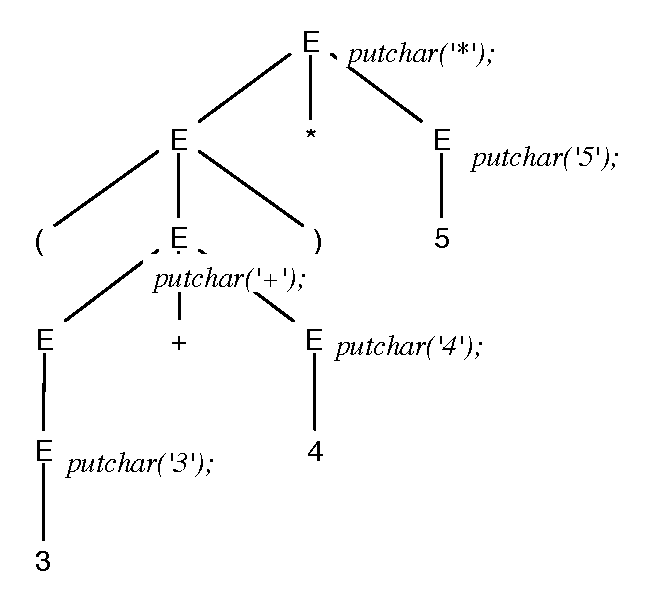
\includegraphics{figure/parse_tree_with_program.pdf}
 \end{center}
 \caption{$(3+4)*5$に対するプログラム断片付き解析木}
 \label{142037_4Apr06}
\end{figure}

得られた解析木を深さ優先でたどり、節点にプログラム断片が付いている場合は
帰りがけにその断片を実行する。すると図\ref{142037_4Apr06}の例では
$3~4~+~5~*$となり、後置記法の式が正しく得られる。

\section{翻訳スキーム}
\label{195223_17Apr06}

図\ref{142037_4Apr06}の例ではプログラム断片を帰りがけに実行したが、一般に
は、行きがけや通りがけにプログラム断片を実行したいこともある。そこで、
\eqref{135829_4Apr06}のプログラム断片付きの文法を少し拡張しよう。これが
{\bfseries 翻訳スキーム}と呼ばれるものである。

\begin{definition}
 文脈自由文法$G$において、$G$の各生成規則の右辺にプログラム断片を埋め込ん
 で得られる(拡張された)文法を{\bfseries 翻訳スキーム}(translation
 scheme)という。翻訳スキームの基になる文脈自由文法$G$を{\bfseries 基底
 文法}(underlying grammar)、埋め込まれたプログラム断片を{\bfseries 意
 味動作}(semantic action)とそれぞれ言う。$\Box$
\end{definition}

\begin{example}
 次に示すのは、基底文法を\eqref{135829_4Apr06}とし、中置記法の式を後置記
 法に変換する翻訳スキームである。
 \begin{equation}
\begin{split}
  E & \rightarrow E + E\ \{ putchar('+'); \} \\
  E & \rightarrow E - E\ \{ putchar('-'); \} \\
  E & \rightarrow E \ast E\ \{ putchar('*'); \} \\
  E & \rightarrow E\ /\ E\ \{ putchar('/'); \} \\
  E & \rightarrow (E) \\
  E & \rightarrow 0\ \{ putchar('0'); \} \\
  \cdots \\
  E & \rightarrow 9\ \{ putchar('9'); \}
\end{split}\label{151014_4Apr06} 
\end{equation}$\Box$
\end{example}

意味動作を特殊な終端記号とみなすと、翻訳スキームは文脈自由文法と見ること
ができ、(意味動作を含んだ)解析木を生成したり、左再帰の除去などの文脈自
由文法の変形手法をそのまま適用したりできる。

\begin{example}
 \eqref{151014_4Apr06}の翻訳スキームを用いて式$4 + 3 * 5$の(意味動作を含
 んだ)解析木を生成すると図\ref{152516_4Apr06}のようになる。この解析木を
 深さ優先にたどり、意味動作の節点ではその意味動作を実行すると、式
 $4~3~5~\ast~+$という後置記法の式が得られる。
\end{example}

\begin{figure}
 \begin{center}
  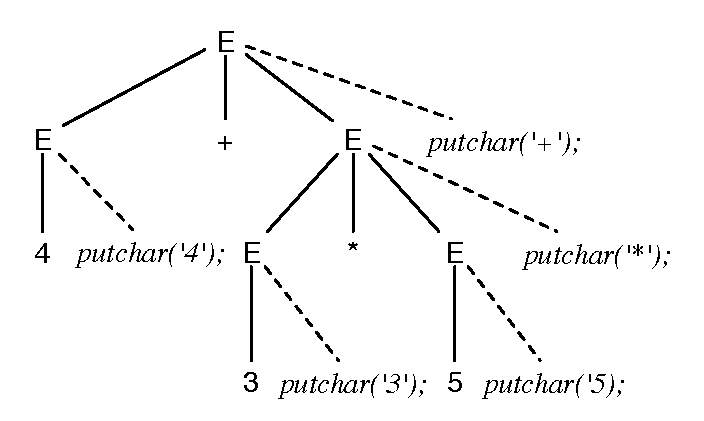
\includegraphics{figure/translation_scheme_parse_tree.pdf}
 \end{center}
 \caption{翻訳スキームによる$4+3*5$の解析木}
 \label{152516_4Apr06}
\end{figure}

\begin{example}
 \eqref{151014_4Apr06}の翻訳スキームに\ref{121145_31Mar06}の手法を適用し
 て左再帰を除去すると、次のような翻訳スキームに変形される。
 \begin{align*}
  E \rightarrow & (E)E' \\
     & \mid 0\ \{ putchar('0'); \}\ E' \\ 
     & \mid \cdots \\
     & \mid 9\ \{ putchar('9'); \}\ E' \\
  E' \rightarrow & +E\ \{ putchar('+'); \}\ E' \\
     & \mid -E\ \{ putchar('-'); \}\ E' \\
     & \mid \ast E\ \{ putchar('\ast'); \}\ E' \\
     & \mid /E\ \{ putchar('/'); \}\ E' \\
     & \mid \epsilon
 \end{align*}
 これを用いて式$3 * (1 + 2)$の解析木を生成すると図\ref{155248_4Apr06}のよ
 うになる。
\end{example}

\begin{figure}
 \begin{center}
  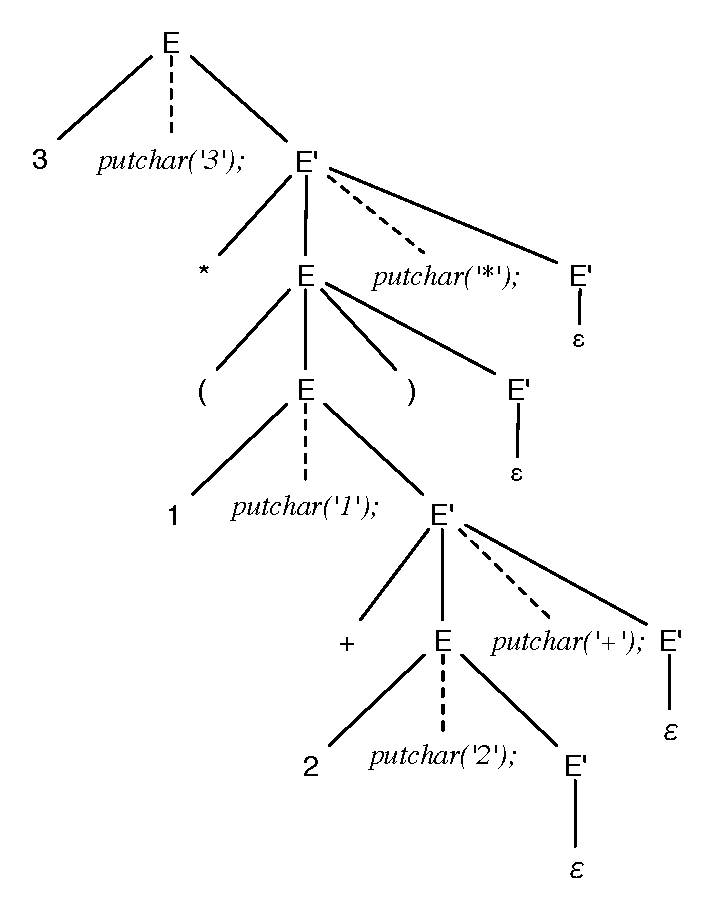
\includegraphics{figure/translation_scheme_no_left_recurs.pdf}
 \end{center}
 \caption{\eqref{151014_4Apr06}による$3 * (1 + 2)$の解析木}
 \label{155248_4Apr06}
\end{figure}

\subsection{意味動作の形式}

以降の節の準備として、意味動作の形式についてもう少し詳しく述べる。これま
で、意味動作はプログラム断片だとしてきたが、どんな形のプログラムでも認め
られるわけではない。使える変数に関して制限がある。

プログラム断片中で使える変数は$X.v$という形式に限られる。ここで$X$は、基
底文法に出現する非終端記号または終端記号である。$v$は翻訳スキーム内で適当
に決めて構わない。$v$を$X$の{\bfseries 属性}(attribute)という。

\section{性質のよい翻訳スキーム}

前節で述べた翻訳スキームによる計算は、常に効率よく行えるわけではない。計
算効率のポイントの一つが「深さ優先に1回たどるだけで計算できるか」である。
解析木は一般に大きくなりがちなので、深さ優先探索の回数が増えるほど、計算
効率が悪くなることが予想されるからである。

そこでこの節では、翻訳スキームの意味動作に制限を加え、深さ優先に1回たどる
だけで計算が行える翻訳スキーム(S属性定義、L属性定義)を導入する。

\subsection{合成属性と相続属性}

もともとの翻訳スキームでは、基底文法に出現する非終端記号や終端記号の属性
はすべて意味動作内で用いることができる。しかし、これでは意味動作の右辺値
($v=E$の形の文の$E$)を計算するのに、解析木のあちこちを参照しなくてはな
らず、深さ優先に1回たどるだけでは到底計算が終わらない。

そこで、性質のよい属性を2つ定義しよう。
\begin{definition}
 解析木の節点$A$について、$A$の属性$x$が$A.x = f(c_1, c_2, \cdots, c_n)$
 と計算できるとする。$c_1, c_2, \cdots, c_n$がすべて$A$の子
 節点の属性であるとき、$x$を$A$の{\bfseries 合成属性}(synthesized
 attribute)という。$\Box$
\end{definition}

\begin{definition}
 解析木の節点$A$について、$A$の属性$x$が$A.x = f(c_1, c_2, \cdots, c_n)$
 と計算できるとする。$c_1, c_2, \cdots, c_n$がすべて$A$の親節点または兄弟
 節点の属性であるとき、$x$を$A$の{\bfseries 相続属性}(inherited
 attribute)という。$\Box$
\end{definition}

生成規則$A \rightarrow \alpha$に基づいて説明すると、次のようになる。
\begin{itemize}
 \item $A$の属性$x$が$\alpha$中の非終端記号や終端記号の属性のみから計算で
       きるなら、$x$は合成属性
 \item $\alpha$中の記号$B$の属性$y$が、$A$や$\alpha$中の他の記号の属性の
       みから計算できるなら、$y$は相続属性
\end{itemize}

\begin{example}
 次に示す翻訳スキームは合成属性のみからなる。添字の$l, r$は、それぞれ左辺
 に出現する記号、右辺に出現する記号を表している。
 \begin{align*}
 E & \rightarrow E + T && \{ E_l.val = E_r.val + T.val; \} \\
 E & \rightarrow T && \{E.val = T.val; \} \\
 T & \rightarrow T * F && \{ T_l.val = T_r.val * F.val; \} \\
 T & \rightarrow F && \{ T.val = F.val; \} \\
 F & \rightarrow (E) && \{ F.val = E.val; \} \\
 F & \rightarrow digit && \{ F.val = digit.lexval; \}
 \end{align*}$\Box$
 \label{example:S-attributed definition}
\end{example}

\begin{example}
 次に示す翻訳スキームのうち、非終端記号$L$の属性$in$は相続属性である。
 \begin{align*}
 D & \rightarrow T\ L && \{ L.in = T.type; \} \\
 T & \rightarrow int && \{ T.type = integer; \} \\
 T & \rightarrow float && \{ T.type = float; \} \\
 L & \rightarrow L, id	&& \{ L_r.in = L_l.in; addtype(id.entry, L_l.in); \} \\
 L & \rightarrow id && \{ addtype(id.entry, L.in); \}
 \end{align*}$\Box$
 \label{example:L-attributed definition}
\end{example}

合成属性や相続属性は、解析木の深さ優先探索と相性が良い。合成属性の計算は、
帰りがけに行うとたどりを1回で済ませることができる。また、相続属性の一部も、
1回のたどりで計算を行うことができる。

\subsection{S属性定義}

\begin{definition}
 翻訳スキームのうち、次の条件を満たすものを{\bfseries S属性定
 義}(S-attributed definition)という。
 \begin{enumerate}
  \item 意味動作中に現れる変数はすべて合成属性である。
  \item すべての意味動作は、生成規則の右辺の末尾にしか現れない。
 \end{enumerate}$\Box$
\end{definition}

\begin{example}
 例\ref{example:S-attributed definition}の翻訳スキームはS属性定義である。
 $\Box$
\end{example}

定義より、S属性定義の意味動作は、解析木を1回深さ優先にたどるだけですべて
計算することができる。

\subsection{L属性定義}

\begin{definition}
 翻訳スキームのうち、次の条件を満たすものを{\bfseries L属性定
 義}(L-attributed definition)という。
 \begin{enumerate}
  \item 意味動作中に現れる変数はすべて合成属性か相続属性である。
	\label{153250_7Apr06}
  \item 基底文法の生成規則$A \rightarrow X_1X_2\cdots X_n$について、
	$X_j$の相続属性は、$X_1, X_2, \cdots, X_{j-1}$の属性と$A$の相続属
	性だけに依存する。
  \item 基底文法の生成規則$A \rightarrow X_1X_2\cdots X_n$について、
	$X_j$の相続属性を左辺に持つ文を含む意味動作は、$X_j$の直前に出現
	する。
  \item 基底文法の生成規則$A \rightarrow X_1X_2\cdots X_n$について、$A$の
	合成属性はこの規則の末尾に出現する。
	\label{153257_7Apr06}
 \end{enumerate}$\Box$
 \label{def:L-attributed definition}
\end{definition}

\begin{example}
 次の翻訳スキームはL属性定義である。ここで、$type$は合成属性、$in$は相続
 属性である\footnote{この翻訳スキームは、\icode{int i, j;} のように
 \icode{int}型の変数を複数同時に宣言するときに、\icode{i}, \icode{j}の型
 を\icode{int} と定めるものである。}。また$entry$は識別子を表す終端記号
 $id$の属性であり、その識別子の名前を格納しているとする。$entry$の値は意
 味解析以前にすでに分かっているものとする。関数$addtype(id.entry, L.in)$
 は、$id.entry$の型として$L.in$を登録する、という動作をする。
 \begin{align*}
  D & \rightarrow T\ \{ L.in = T.type; \}\ L \\
  T & \rightarrow \icode{int}\ \{ T.type = integer; \} \\
  T & \rightarrow \icode{float}\ \{ T.type = float; \} \\
  L & \rightarrow \{ L_r.in = L_l.in; \}\ L\ \icode{,}\ \icode{id}\ \{ addtype(\icode{id}.entry, L_l.in); \}\\
  L & \rightarrow \icode{id}\ \{ addtype(\icode{id}.entry, L.in); \}
 \end{align*}$\Box$
 \label{example:L-attributed translation scheme}
\end{example}

定義\ref{def:L-attributed definition}の\ref{153250_7Apr06}と
\ref{153257_7Apr06}から分かるように、もしL属性定義に相続属性が一つも含ま
れなければ、S属性定義そのものである。すなわち、S属性定義は必ずL属性定義に
なる。

S属性定義と同様に、L属性定義の翻訳スキームも解析木を1回深さ優先にたどるだ
けで、すべての意味動作を計算することができる。

\begin{figure}
 \begin{center}
  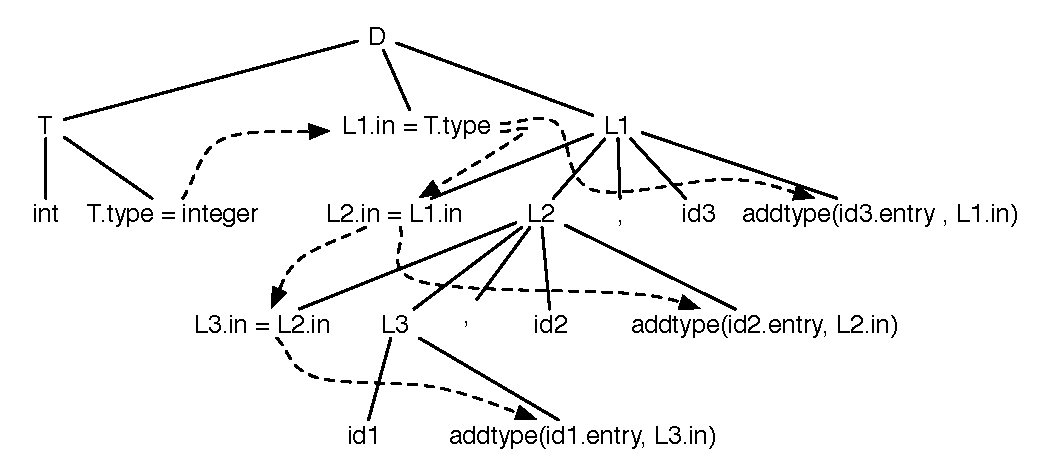
\includegraphics[width=13cm]{figure/L_attr_translation_scheme.pdf}
 \end{center}
 \caption{L属性定義に基づく解析木}
 \label{170525_7Apr06}
\end{figure}

\begin{example}
 例\ref{example:L-attributed translation scheme}の翻訳スキームに基づいて、
 トークン列\icode{int id, id, id}から生成した意味動作付き解析木を図
 \ref{170525_7Apr06}に示す。なお、非終端記号$L$、終端記号$id$が複数現れる
 ので、便宜上添字を付けて区別している。

 図中の破線は、属性の依存関係を示している。例えば、意味規則$T.type =
 integer;$で決定した$T.type$の値を$L_1.in = T.type;$で参照する、といった
 具合である。この解析木を深さ優先でたどっていくと、破線で示した属性の依存
 関係の順序を守りながら意味規則が計算されていくことを確かめよ。$\Box$
\end{example}

% \section{翻訳スキームを実行するプログラムの生成}

% 一般には、翻訳スキームを実行するプログラムを生成するのは単純ではない。し
% かし、基底文法をLL(1)文法など予測型構文解析の行える文法に制限し、かつ翻訳
% スキームをS属性定義・L属性定義に制限すると、翻訳スキームを実行するプログ
% ラムは自動生成できる。

% 予測型構文解析ルーチンは次のように生成するのであった。
% \begin{enumerate}
%  \item 各非終端記号に対応する関数を用意する
%  \item その関数内に、生成規則の右辺にならって、節点の生成や非終端記号に対
%        応する関数呼び出しを並べる
%        \label{153525_10Apr06}
% \end{enumerate}
% これを実行すると、あたかも解析木を深さ優先にたどるように処理が行われる。

% そこで、\ref{153525_10Apr06}を行うときに、意味動作を対応する場所に埋め込
% む。すると、得られた予測型構文解析ルーチンを実行すると、解析木を深さ優先
% でたどりながら対応する意味動作が実行され、S属性定義やL属性定義であれば正
% しく処理されることになる。

% ただし、

% - [ ] 予測型構文解析への翻訳スキームの埋め込み
% 	- [ ] 例:2-13(合成属性も相続属性も含まれていない)
% 	- [ ] 左再帰の除去
% 		- [ ] 生成規則の中に埋め込んだ意味動作も一緒に行う
% 		- [ ] 2-13 → 2-14、翻訳の様子:図2.21
% 	- [ ] 翻訳プログラムの生成
% 		- [ ] 予測型構文解析と同様
% 		- [ ] 意味動作に対応する場所に、意味動作のプログラム片をそのまま埋め込む
% 		- [ ] 結果:2-22
% - [ ] 一般的な翻訳スキームの埋め込み
% 	- [ ] 合成属性も相続属性も含まれる場合
% 	- [ ] ポイント:意味動作の中で参照する属性は、その動作を実行する時点ではすでに評価し終わっていなければならない(値が求まっていなければならない)
% 		- [ ] 生成規則の右辺の記号の相続属性:その記号より前の動作で値が求められていなければならない
% 		- [ ] 各動作の中では、その動作より右にある記号の合成属性を参照してはいけない
% 		- [ ] 生成規則の左辺の非終端記号の合成属性:参照する属性をすべて計算した後、計算する(意味動作を生成規則の右辺の最後に置く)
% 	* [ ] 構文主導定義から翻訳スキームを作るには
% 	- [ ] 左再帰の除去
% 		- [ ] 上の3つの条件を満たすように、意味動作を変形しなければならない
% 		- [ ] 5-24→ 5-25
% 			- [ ] 新たに導入された非終端記号 R, R1の属性 i, s
% 		- [ ] 抽象的には
% 			- [ ] 翻訳スキーム変換
% 			- [ ] 属性値の求め方の違い:図5.27
% 		- [ ] 予測型構文解析ルーチン+翻訳スキーム埋め込み の生成
% 			- [ ] 非終端記号Aに対する関数 A()
% 				- [ ] Aの相続属性を仮引数に
% 				- [ ] Aの合成属性を返り値に
% 				- [ ] Aを左辺とする生成規則に現れる記号の属性を局所変数に
% 			- [ ] 生成規則の右辺を左から右に調べ
% 				- [ ] 合成属性 x を持つトークン(終端記号)X
% 					- [ ] X.xに対応する変数 = X.xの値; Xとの照合; 入力を先に進める;
% 				- [ ] 非終端記号B
% 					- [ ] Bの合成属性に対応する変数 = B(b1, b2, …, bk);
% 						- [ ] b1, b2, …, bk:Bの相続属性に対応する変数
% 				- [ ] 意味動作
% 					- [ ] プログラム片を複写(属性の参照は、対応する変数の参照に置き換え)
% 			- [ ] 例:5-31

